\documentclass[a4paper,11pt]{scrartcl}

\usepackage{biblatex}
\usepackage{lmodern}
\usepackage[T1]{fontenc}
\usepackage[a4paper, total={14cm, 24cm}]{geometry}
\usepackage{textcomp}
\usepackage{gensymb}
\usepackage{graphicx}
\usepackage{float}
\usepackage{caption}
\usepackage{hyperref}
\usepackage{paralist}
\usepackage{xcolor}
\usepackage{subcaption}
\usepackage[font={footnotesize,it}]{caption}
\usepackage{amsmath,amssymb,amsthm} 
\usepackage{url}
\usepackage{xspace}
\usepackage{algorithmic}
\usepackage{mathpazo}
\usepackage{booktabs}
\usepackage{subfiles}
\usepackage{silence}

% [Settings]

\WarningFilter{DuplicateLabels}

\newcommand{\ie}{ie}
\newcommand{\eg}{eg}
\newcommand{\reffig}[1]{Figure~\ref{#1}}
\newcommand{\refsec}[1]{Section~\ref{#1}}

\setcapindent{1em} %-- for captions of Figures
\setlength\parskip{1em plus 0.1em minus 0.2em}
\setlength\parindent{0pt}
\sffamily

\renewcommand{\algorithmicrequire}{\textbf{Input:}}
\renewcommand{\algorithmicensure}{\textbf{Output:}}

\addbibresource{ref.bib}

% [Title Page] (could be split away)

\titlehead{\centering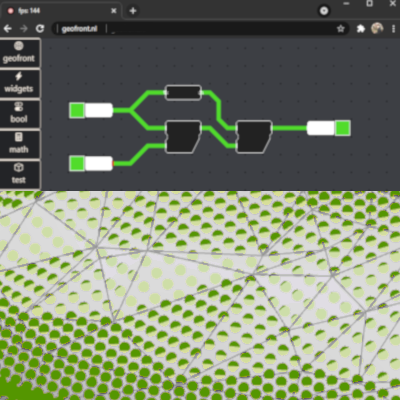
\includegraphics[width=12cm]{images/thumbnail.png}}
\title{Thesis Proposal: \\
Client-side geo-processing using WebAssembly and Visual Programming
}

\author{
  Jos Feenstra\\
  student \#4465768 \\
  \url{me@josfeenstra.nl}\\
  \\
  1st supervisor: Stelios Vitalis \\
  2nd supervisor: Ken Arroyo Ohori \\
}

\date{November, 2021}

\begin{document}

\clearpage\maketitle
\thispagestyle{empty}
\sffamily

\begin{center}
  \textbf{Key words:} Geomatics, WebAssembly, 3D geometry, Geodata, Visual programming, 
\end{center}

% [Table of Content] 
\newpage
\tableofcontents

% [Body]
\newpage
%-------------------------------------------------------------------------------------------------%
% An introduction in which the relevance of the project and its place in the 
% context of geomatics is described, along with a clearly-defined problem statement.
\section{Introduction}

% [1]
\par
Geodata processing is important.

% [2]
% [JF]: This is nice, By 'improving a VPL' I dont have to go all 'use case testing' and make a case for a vpl, 
% because I can just state in this introduction "they are useful, look, multiple people are working on them"
\par
Visual programming languages, or Vpl's for short, can make geodata processing debugable and more insightful. 

[Name some relevant VPL's, their reason of existence, their target audience.
this will be more in-depth during the 'related work' section] 


% [3]
% [JF]: these criteria are Ideals, of course software falls short on meeting them, make this more nuanced)
\subsection{Problem}
The main advantage of vpl's is usability. 
However, vpl's used within the field of geomatics still fall short on certain usability aspects. 
The well established FAIR paradigm has been used to judge the usability of geodata, and geodata portals (SOURCE: GEOLEGAL). 
This paper will use this paradigm instead on vpl's, for geodata processing itself can have varying degrees of Findability, Accessibility, Interoperability, and Reusability. 
When we judge the aforementioned vpl's on these aspects, compared to regular programming languages we find the following: 


\subsubsection*{Accessibility}
Accessibility is arguably the strongest advantage of a visual programming language over a regular language. 
Users whom are not familiar with programming can often still use a VPL. 
However, many VPL's are still hard to actually acquire. 
The tool needs to be installed, an account is required, and most VPL's are not free and open source like the vast majority of programming languages are. (Study on advantage of web-based tools over native ones)

\subsubsection*{Interoperability}
Besides a large barrier of entry, Visual programming languages are also not platform agnostic. 
\dots
are usually strongly tied to their host environments
\dots
This also makes Bindings to different languages or programs harder. A regular programming language like python can accepts bindings, which makes it possible to run scripts written in C++ or Rust. Similar actions are often difficult to accomplish with VPL's.

\subsubsection*{Findability}
It is often hard to get an overview of 


\subsubsection*{Reusability}
Reusability is arguably a core concept within computer programming in general. 
A function is defined with the idea that it may be used multiple times, in multiple different contexts, with a variety of different input data.
Vpl's are often not as reusable as 'normal' code. The flowchart-scripts often cannot be turned into standalone applications or tools.



% [5] go from this to research question
\newpage
\subsection{Solution}


\subsubsection*{Accessible}


\subsubsection*{Interoperable}



\subsubsection*{Findable}


\subsubsection*{Reusable}



\newpage
%-------------------------------------------------------------------------------------------------%
% A related work section in which the relevant literature is presented and 
% linked to the project. 
% It should show that you clearly know the problem you plan to solve, 
% and that you master the related work. 
\newpage
\section{Related work}

\subsection{On VPLs}
Lots of research has been done on the topic of VPL's, and their advantages and disadvantages. 
(I explicitly want to name the cognitive dimentions paper, it is very good and appropriate, and contains many suggestions for future VPL's)


\subsection{On geo web processing services}
These are client-side interfaces for server side processes. 
Due to the massive nature of geodata, this is understandable.


\subsection{On WebAssembly}
I found a couple of interesting papers on WebAssembly, including the original wasm paper



\subsubsection*{Existing Geo Information applications utilizing WebAssembly}

\begin{itemize}
  \item Google earth
  \item the cityjson validator
\end{itemize}
\newpage
%-------------------------------------------------------------------------------------------------%
% [HUGO]: The research questions are clearly defined, along with the scope (ie what you will not be doing).
% To help you define a "good" research question, 
% read \url{https://sites.duke.edu/urgws/files/2014/02/Research-Questions_WS-handout.pdf}.
% [ From Hugo's handout: ]
% 
% clear | focussed | unique | 
% start asking open-ended “How?” “What?” and Why?” questions. 
% Then evaluate possible responses to those questions
% While a good research question allows the writer to take an arguable position, 
% it DOES NOT leave room for ambiguity.
% 
% 1)Is the research question something I/others care about? Is it arguable?
% 2)Is the research question a new spin on an old idea, or does it solve a problem?
% 3)Is it too broad or too narrow?
% 4)Is the research question researchable within the given time frame and location?
% 5)What information is needed?
% 
% are you trying to accomplish one of these goals? 
% 1) Define or measure a specific fact or gather facts about a specific phenomenon. -> NO
% 2) Match facts and theory. -> NO
% 3) Evaluate and compare two theories, models, or hypotheses. -> NO
% 4) Prove that a certain method is more effective than other methods. -> ONLY WASM compared to native
% Moreover, the research question should address what the variables of the experiment are, their relationship, 
% and state something about the testing ofthose relationships. 
% 
% [JF] : I really know what I want to do, and I am convinced improving the usability of geoprocessing tools is both valuable and Good. 
% 
\newpage
\section{This Study}

The aim of this study is to provide an environment meant for client-side geoprocessing using WebAssembly. 
This environment will be used to demonstrate if and how wasm-based, client-side geoprocessing is possible. 
At the same time, by presenting this environment, the study aims to explore the functionality and design possibilities of a web-GIS application equipped with such tools. 

This will require research into the technical effectiveness of WebAssembly. 
C++ geoprocessing libraries such as CGAL \& GDAL will be tested on their ability to be compiled, loaded, and used from a browser. 
This is compared against their compilation by other means, such as native binaries or the aforementioned `asm.js`. 

This research is complemented by an extensive 'case study' to explore the design possibilities of a web-application equipped with client-side geoprocessing. 
A thick-client web application will be created, and this will serve as platform for testing the aforementioned `wagl`'s. 
The tool and can be additionally used for acquiring, visualizing, and saving geodata. 

% (WebAssembly geoprocessing libraries -> `wagl`'s)

%-------------------------------------------------------------------------------------------------%
\subsection{Research Questions}



\subsubsection*{Sub Questions}



% ----
\newpage
\subsection{Scope (\& Method?)}


\subsection*{Will Include}

\subsubsection*{Benchmarks of C++ geoprocessing libraries native versus wasm}

The performance benefits of WebAssembly are an important component of why WebAssembly might be beneficial for client-side geoprocessing. As such, this research is interested in confirming whenether this is the case for geoprocessing applications. Individual functions of geoprocessing libraries will be benchmarked using five different methods: 

\begin{itemize}
    \item Compiled and run as native binary (g++), 
    \item Compiled to wasm, run natively (WASI),
    \item Compiled to wasm, run in a browser,
    \item Compiled to asm.js, run natively (NODE.js),
    \item Compiled to wasm, run in a browser. 
\end{itemize}


\subsubsection*{Comparison and discussion of multiple wasm compilation methods for large libraries}
This research will try out multiple methods of WASM compilation. 
Since compiling and downloading full libraries might become very slow, We might need to look at incremental methods of compiling and distributing libraries. 
This is possible since Wasm libraries do accept dependencies. 
Additionally, 


\subsubsection*{Implementation details of creating a geo-web-vpl}

This study will include implementation details of the VPL, and the design considerations made during its development. These decisions will be informed by analysis of exsting geo-vpl's, and studies discussing the usability aspects of VPL's (SOURCE: VPL Usability paper,  Ravi Peter)


\subsubsection*{Conclusions and Discussion on using WebAssembly for geo-processing}

Additionally, this study will give an answer to if and how WebAssembly contributed to performant and sharable geoprocessing. 
This will be based on the aforementioned quantitative assessment of performance and compilation possibilities, but also on the experience gathered by using the built application.  

\subsubsection*{Conclusions and Discussion on using a web based VPL for geo-processing}

Additionally, this study will give an answer to if and how a VPL contributed to more usable geoprocessing. This will be a purely qualitative assessment, based on the findings and experience using the environment.  


%-----------------------------------------------------------------------------%
\subsection*{Will not include}

\subsubsection*{Server-side WebAssembly} % **Client-side WebAssembly Only**

This study will limit itself to the **client-side** usage of WebAssembly. 
A powerful case can be made for **server-side** usage of WebAssembly, especially in conjunction with a programming language such as Rust. 
Rust compiled to WebAssembly could, compared to using python, java or C++, make geoprocessing more maintainable and reliable, while at the same time ensuring memory safety, security, and performance [SOURCE: wasi, wasm-ai]. 
Server-side wasm is beyond the scope of this paper, but would be an excellent starting point for future work. 

Note that this also means that research into `wagl`'s is important for more than just client-side geoprocessing. All geoprocessing could benefit from it.



\subsubsection*{Web Processing Services} % Will not be dealing with WPS 

This research will exclude the OGC standard of web processing services (SOURCE), since these services are not about \emph{client} side geoprocessing, but instead cover \emph{server} side geoprocessing. 
Future work could, however, research the possibility of utilizing a vpl for WPS orchestration. 



\subsubsection*{Usability Analysis of geoprocessing VPL's} % 

While usability* is a primary motivation for conducting this research, no claims will be made that a client-side vpl geoprocessing environment is more usable to native GIS applications or geoprocessing methods. This research attempts to solve practical inhibitions in order to discover whether or not client-side is \textbf{an} option. If it turns out that this method is viable technically, future research will be needed to definitively proof \textbf{how} usable it is compared to all other existing methods.  

% This paper seeks to first close this gap, limiting itself to overcoming the technical and design boundaries in the pursuit of practical client-side geoprocessing.

* (Usability within this context is meant as a collection of aspects such as "performance", "ease of use", and FAIR principles. )

Similarly, a survey analyzing how users experience client-side geoprocessing in comparison to native geoprocessing must also be left to subsequent research. While this would gain us tremendous insight, client-side geoprocessing is too new to make a balanced comparison. Native environments like GRASSGIS, QGIS, FME or Esri simply have a 20+ year lead in research and development. 





% ### This Study

% The aim of this study is to provide an environment meant for client-side geoprocessing using WebAssembly. This environment will be used to demonstrate if and how wasm-based, client-side geoprocessing is possible. At the same time, by presenting this environment, the study aims to explore the design possibilities of a web-GIS application equipped with such tools. 

% This will require research into the technical effectiveness of WebAssembly. C++ geoprocessing libraries such as CGAL & GDAL will be tested on their ability to be compiled, loaded, and used from a browser. This is compared against their compilation by other means, such as native binaries or the aforementioned `asm.js`. This research is complemented by an extensive 'case study' to explore the design possibilities of a web-application equipped with client-side geoprocessing. A thick-client web application will be created, and this will serve as platform for testing the aforementioned `wagl`'s. The tool and can be additionally used for acquiring, visualizing, and saving geodata. 

% (WebAssembly geoprocessing libraries -> `wagl`'s)

% <br><br><br>

% ### Limits & Future Work

% **Client-side WebAssembly Only**

% This study will limit itself to the **client-side** usage of WebAssembly. A powerful case can be made for **server-side** usage of WebAssembly, especially in conjunction with a language like Rust. WebAssembly + Rust could, compared to using python, java or C++, make geoprocessing more maintainable and reliable, while at the same time ensuring memory safety, security, and performance [SOURCE: wasi, wasm-ai]. Server-side wasm is beyond the scope of this paper, but would be an excellent starting point for future work. 

% Note that this also means that research into `wagl`'s is important for more than just client-side geoprocessing. All geoprocessing could benefit from it.

% **No Surveys**

% Additionally, a survey analyzing how users experience client-side geoprocessing in comparison to native geoprocessing must also be left to subsequent research. While this would gain us tremendous insight, client-side geoprocessing is insufficiently researched and developed to make a balanced comparison. Native environments like GRASSGIS, QGIS, FME or Esri simply have a 20+ year lead. This paper seeks to first close this gap, limiting itself to overcoming the technical and design boundaries in the pursuit of practical client-side geoprocessing. It seeks to present client-side geoprocessing as **an** option. Afterwards, Future research will have to be done to discover if this is **the** option (for a particular use case). 
\newpage
%-------------------------------------------------------------------------------------------------%
% This is not an official section, but important nonetheless
\newpage
\section{Motivation}



\newpage
%-------------------------------------------------------------------------------------------------%
% Overview of the methodology to be used.
\newpage
\section{Methodology}
This research attempts to improve the Accessibility and Interoperability issues of VPL's by developing a prototype VPL. 
This prototype will be used as the stage to develop the tools and knowledge necessary to utilize the Web \& WebAssembly for geodata processing.   

\par
A logbook will be maintained to explain how this prototype was constructed, what design choices were made and why, and exactly in which way the FAIR principles influenced its design. 

\par
When the VPL contains all tools necessary to be used to properly process geodata, a final assessment is needed. 
Three different applications will be created using regular means (jupyter notebook, python, panda's, etc)
and these same applications will be created using the prototype web-VPL. 
These two methods will then be compared on usability aspects and performance.   

Case Study
\newpage
%-------------------------------------------------------------------------------------------------%
% Having a Gantt chart is probably a better idea then just a list.
\newpage
\section{Time planning}

todo
\begin{itemize}
    \item write P2
    \item write P2 presentation
    \item build the VPL
    \item apply VPL to Case Study
    \item build a similar application using python + jupyler, or some other conventional method
    \item perform tests and compare the two
\end{itemize}



% start with a todo list 
% make workload estimations


\newpage
%-------------------------------------------------------------------------------------------------%
% Since specific data and tools have to be used, it’s good to present these concretely, 
% so that the mentors know that you have a grasp of all aspects of the project.
\newpage
\section{Tools and data}

\subsubsection{Tools}

In order to develop a web-based geo-vpl, several tools will be required. 

\begin{itemize}
  \item Typescript
  \item 3D visualization using webgl 
  \item WebAssembly
  \item C++ 
\end{itemize}


?? for judging other geo-vpls: 
\begin{itemize}
  \item FME
  \item Geoflow
  \item Grasshopper
  \item ...
\end{itemize}


\subsubsection{Data}

Data for the case study:
\begin{itemize}
  \item WMS \& WFS services hosted by PDOK.
\end{itemize}


% [Appendix]
\newpage
\printbibliography

\end{document}